\documentclass[14pt]{extarticle} 
\usepackage{amsmath,mathtools,amsfonts,amsthm,amssymb,hyperref}
\usepackage{wasysym,geometry,bussproofs,latexsym,parskip,bookmark}
\usepackage{mathtools,float}
\newtheorem{defn}{Definition}
\newtheorem{thm}{Theorem}
\newtheorem{claim}{Claim}
\newtheorem{lemma}{Lemma}
\newcommand{\dps}{\displaystyle}
\hypersetup{colorlinks,allcolors=blue,linktoc=all}
\geometry{a4paper} 
\geometry{margin=0.5in}
\title{Math for CS 2015/2019 solutions to ``In-Class Problems Week 31, Mon. (Session 31)''}
\author{https://github.com/spamegg1}
\begin{document}
\maketitle
\tableofcontents

\section{Problem 1}
Guess the Bigger Number Game

Team 1:

Write two different integers between 0 and 7 on separate pieces of paper.

Put the papers face down on a table.

Team 2:

Turn over one paper and look at the number on it.

Either stick with this number or switch to the other (unseen) number.

Team 2 wins if it chooses the larger number; else, Team 1 wins.

The analysis given before class implies that Team 2 has a strategy that wins 4/7 of the time no matter how Team 1 plays. Can Team 2 do better? The answer is “no,” because Team 1 has a strategy that guarantees that it wins at least 3/7 of the time, no matter how Team 2 plays. Describe such a strategy for Team 1 and explain why it works.

\begin{proof}
Team 1 should randomly choose a number $Z \in \{0, \ldots, 6\}$ and write $Z$ and $Z + 1$ on the pieces of paper with all numbers equally likely.

To see why this works, let $N$ be the number on the paper that Team 2 turns over, and let OK be the event that $N \in \{1, \ldots, 6\}$. So given event OK, that is, given that $N \in \{1, \ldots, 6\}$, Team 1’s strategy ensures that half the time $N$ is the higher number and half the time $N$ is the lower number. So given event OK, the probability that Team 1 wins is exactly 1/2 no matter how Team 2 chooses to play (stick or switch).

Now we claim that Pr[OK] = 6/7 which implies that the probability that Team 1 wins is indeed at least (1/2)(6/7) = 3/7.

To prove Pr[OK] = 6/7, we can follow the four step method. (Note that we couldn’t apply this method to model the behavior of Team 2, since we don’t know how they may play, and so we can’t let our analysis depend on what they do.)

The first level of the probability tree for this game will describe the value of $Z$: there are seven branches from the root with equal probability going to first level nodes corresponding to the seven
possible values of $Z$. The second level of the tree describes the choice of the number, $N$: each of the seven first-level nodes has two branches with equal probability, one branch for the case that
$N = Z$ and the other for the case that $N = Z + 1$. So there are 14 outcome (leaf) nodes at the second level of the tree, each with probability 1/14.

\begin{figure}[ht!]
\centering
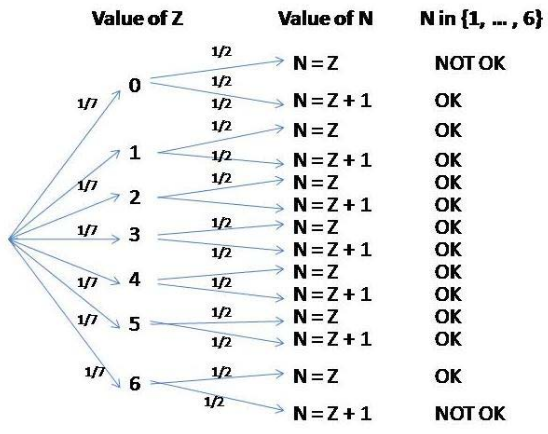
\includegraphics[scale=0.6]{guess-game.png}
\end{figure}

Now only two outcomes are not OK, namely, when $Z = 6$ and $N = 7$, and when $Z = 0$ and $N = 0$. Each of the other twelve outcomes is OK, and since each has probability 1/14, we conclude that Pr[OK] = 12/14 = 6/7, as claimed.
\end{proof}

\section{Problem 2}
Let $I_A$ and $I_B$ be the indicator variables for events $A$ and $B$. Prove that $I_A$ and $I_B$ are independent iff $A$ and $B$ are independent.

Hint: Let $A^1 \Coloneqq A$ and $A^0 \Coloneqq\overline{A}$, so the event $[I_A = c]$ is the same as $A^c$ for $c \in \{0,1\}$; likewise for $B^1, B^0$.

\begin{proof}
Assume $I_A$ and $I_B$ are independent. Then

\begin{center}
\begin{tabular}{rclr}
Pr$[A \cap B]$ & = & Pr$[I_A = 1$ AND $I_B = 1]$ & (by definition) \\
& = & Pr$[I_A = 1] \cdot$ Pr$[I_B = 1]$ &(by independence)\\
& = & Pr$[A] \cdot $ Pr$[B]$ & (by definition)
\end{tabular}
\end{center}

Therefore $A$ and $B$ are independent.

Conversely assume $A$ and $B$ are independent. So Pr$[A \cap B]$ $=$ Pr$[A]$ $\cdot$ Pr$[B]$. We need to show that:

1. the events $[I_A = 0]$ and $[I_B = 0]$ are independent,

2. the events $[I_A = 0]$ and $[I_B = 1]$ are independent,

3. the events $[I_A = 1]$ and $[I_B = 0]$ are independent,

4. the events $[I_A = 1]$ and $[I_B = 1]$ are independent.

We will only show (3), because the other three proofs are very similar.

\begin{center}
\begin{tabular}{rclr}
Pr$[(I_A=1) \cap (I_B=0)]$ & = & Pr$[A \cap \overline{B}]$ & (by definition) \\
& = & Pr$[A - B]$ & (by set algebra)\\
& = & Pr$[A]$ $-$ Pr$[A \cap B]$ & (by Difference Rule)\\
& = & Pr$[A]$ $-$ Pr$[A]$ $\cdot$ Pr$[B]$ & (by independence)\\
& = & Pr$[A](1 - $ Pr$[B])$ & (by algebra)\\
& = & Pr$[A]$ $\cdot$ Pr$[\overline{B}]$ & (by Complement Rule)\\
& = & Pr$[I_A=1]$ $\cdot$ Pr$[I_B=0]$ & (by definition)
\end{tabular}
\end{center}

\end{proof}

\section{Problem 3}
Let $R_1, R_2, \ldots, R_m$ be mutually independent random variables with uniform distribution on $[1,n]$. Let $M \Coloneqq \max \{R_i \,\,\, | \,\,\, i \in [1, m]\}$.

\subsection{(a)}
Write a formula for PDF$_M(1)$.

\begin{proof}
We have Pr$[R_i = k] = 1/n$ for all $k \in [1,n]$ and all $1 \leq i \leq m$. The event $M = 1$ is the event that all $m$ variables equal 1, and since they are mutually independent, we have
$$
Pr[M = 1] = Pr[R_1 = 1] \cdot \ldots \cdot Pr[R_m = 1] = \frac{1}{n} \cdot \ldots \cdot \frac{1}{n} = \frac{1}{n^m}
$$
So:
$$
PDF_M(1) = \frac{1}{n^m}
$$
\end{proof}

\subsection{(b)}
More generally, write a formula for Pr$[M \leq k]$.

\begin{proof}
The event $M \leq k$ is the event that all $m$ of the variables are at most $k$, so by mutual independence we have
$$
Pr[M \leq k] = Pr[R_1 \leq k] \cdot \ldots \cdot Pr[R_m \leq k] = \frac{k}{n} \cdot \ldots \cdot \frac{k}{n} = \frac{k^m}{n^m}
$$
\end{proof}

\subsection{(c)}
For $k \in [1,n]$, write a formula for PDF$_M(k)$ in terms of expressions of the form ``Pr$[M \leq j]$'' for $j \in [1, n]$.

\begin{proof}
The event $M = k$ is the event $M \leq k$ minus all the events $M = 1, \ldots, M = k-1$, which is the same as the event $M \leq k-1$. So we have PDF$_M(k)$ = Pr$[M \leq k]$ $-$ Pr$[M \leq k-1]$.
\end{proof}

\section{Problem 4}
Suppose you have a biased coin that has probability $p$ of flipping heads. Let $J$ be the number of heads in $n$ independent coin flips. So $J$ has the general binomial distribution:
$$
PDF_J(k) = \binom{n}{k}p^kq^{n-k}
$$
where $q \Coloneqq 1-p$.

\subsection{(a)}
Show that
$$
\begin{tabular}{lr}
PDF$_J(k-1) < $ PDF$_J(k)$ & for $k < np + p$,\\
PDF$_J(k-1) > $ PDF$_J(k)$ & for $k > np + p$.
\end{tabular}
$$
\begin{proof}
Consider the ratio of the probability of $k$ heads over the probability of $k - 1$ heads.
$$
\begin{array}{rcl}
\dps\frac{PDF_J(k)}{PDF_J(k-1)}&=&\dps\frac{\binom{n}{k}p^k q^{n-k}}{\binom{n}{k-1}p^{k-1} q^{n-k+1}}\\
&=&\dps\frac{n!/[k!(n-k)!]}{n!/[(k-1)!(n-k+1)!]}\cdot \frac{p}{q}\\
&=&\dps\frac{(n-k+1)p}{kq}
\end{array}
$$
This fraction is greater than 1 precisely when $(n - k + 1)p > kq = k(1 - p)$, that is when $k < np + p$. So for $k < np + p$, the probability of $k$ heads increases as $k$ increases, and for $k > np + p$, the probability decreases as $k$ increases.
\end{proof}

\subsection{(b)}
Conclude that the maximum value of PDF$_J$ is asymptotically equal to
$$
\frac{1}{\sqrt{2\pi npq}}
$$

Hint: For the asymptotic estimate, it’s ok to assume that $np$ is an integer, so by part (a), the maximum value is PDF$_J(np)$. Use Stirling’s Formula.

\begin{proof}
$$
\begin{array}{rcl}
PDF_J(np)&\Coloneqq&\binom{n}{np}p^{np}q^{n-np}\\
&=&\dps\frac{n!}{(np)!(nq)!}p^{np}q^{nq}\\
&\sim&\dps\frac{(n/e)^n\sqrt{2\pi n}}{(np/e)^{np}\sqrt{2\pi np} (nq/e)^{nq}\sqrt{2\pi nq}}p^{np}q^{nq}\\
&=&\dps\frac{(n/e)^n\sqrt{2\pi n}}{(n^{np}p^{np}/e^{np})\sqrt{2\pi np} (n^{nq}p^{nq}/e^{nq})\sqrt{2\pi nq}}p^{np}q^{nq}\\
&=&\dps\frac{(n/e)^n\sqrt{2\pi n}}{(n^{np+nq}p^{np}q^{nq}/e^{np+nq})\sqrt{2\pi np}\sqrt{2\pi nq}}p^{np}q^{nq}\\
&=&\dps\frac{(n/e)^n\sqrt{2\pi n}}{(n/e)^n\sqrt{2\pi np}\sqrt{2\pi nq}}\\
&=&\dps\frac{1}{\sqrt{2\pi npq}}
\end{array}
$$
\end{proof}

\section{Problem 5 (Supplemental Problem)}
You have just been married and you both want to have children. Of course, any child is a blessing, but your spouse prefers girls, so you decide to keep having children until you have a girl. In other words, if your 1st child is a girl, you’ll stop there. If it’s a boy, then you’ll have a 2nd child, too. If that one is a girl, you’ll stop there. Otherwise, you’ll have a 3rd child, and so on. Assume that you will never abandon this ingenious plan and that every child is equally likely to be a boy or a girl, independently of the number of its brothers so far. Let $B$ be the boys that you will eventually have to put up with to enjoy the company of your beloved daughter.

\subsection{(a)}
For $i = 0, 1, 2, \ldots,$ what is the value of PDF$_B(i)$?

\begin{proof}
Pr$[B = 0]$ is 1/2, because it happens only when the first child is a girl.

Pr$[B = 1]$ is 1/4, because it happens only when the first child is a boy and the second child is a girl.

Pr$[B = 2]$ is 1/8, because it happens only when the first two children are both boys, and the third child is a girl.

In general Pr$[B = i] = \dps\frac{1}{2^{i+1}}$.
\end{proof}

\subsection{(b)}
For $i = 0, 1, 2, \ldots,$ what is the value of CDF$_B(i)$?

\begin{proof}
Pr$[B \leq 0]$ is 1/2, because it happens only when the first child is a girl.

Pr$[B \leq 1]$ is 3/4, because it happens only when either the first child is a girl, or when the first child is a boy and the second child is a girl.

Pr$[B \leq 2]$ is 7/8, because it happens when either $B = 2$ or $B \leq 1$.

In general Pr$[B \leq i] = \dps\frac{2^{i+1} - 1}{2^{i+1}}$.
\end{proof}
\end{document}
